\section{ Launch Trajectories:T-constant.EOM vertical derive }\label{sec:q4}    

\begin{enumerate}[label=(\alph*)]
\item
We know that $I_{sp}=c_{eff}/g_0$, $\psi_0=\frac{T}{M_0g_0}$ and $T=mc_{eff}$. Constant thrust $\Rightarrow$ Constant mass flow rate. Therefore, the expression for instantaneous mass is
$$M=M_0-mt=M_0-\frac{T}{c_{eff}}t=M_0\left(1-\frac{Tg_0}{M_0g_0c_eff}t\right)$$
$$\Rightarrow M=M_0\left(1-\frac{\psi_0}{I_{sp}}t\right)$$

Total burn time $t_b$ occurs at $M=M_e$ $$t_b=\frac{I_{sp}}{\psi_0}\left(1-\frac{M_e}{M_0}\right)=37.5\: s$$

\item
Equation of vertical motion along the rail
$$M\frac{dV}{dt}=T-Mg_0$$
$$\Rightarrow \frac{dV}{dt}=\frac{T}{M}-g_0$$
Velocity of the rocket
$$\int^V_0 dV = \int_0^t \left(\frac{mc_{eff}}{M}-g_0\right)dt$$
Since, $m=-dM/dt$,
$$V = -\int_{M_0}^M \frac{I_{sp}g_0}{M}dM-\int_0^t g_0dt$$
$$\Rightarrow V = I_{sp}g_0\log\frac{M_0}{M}-g_0t$$

Altitude of the rocket when in guide rail
$$Z=\int_0^t Vdt= \int_0^t (I_{sp}g_0\log\frac{M_0}{M}-g_0t)dt=-\int_{M_0}^M \frac{I_{sp}g_0}{m}log\frac{M_0}{M}dM - \int_0^t g_0tdt$$
$$Z=\frac{I_{sp}^2g_0}{\psi_0}\left[1-\frac{M}{M_0}\left(1+\log\frac{M_0}{M}\right)\right]-\frac{1}{2}g_0t^2$$
To eliminate the t term in the equation, the expression $t=\frac{M_0-M}{m}$ is used.

For the given problem, $$m=T/c_{eff}=\frac{\psi_0M_0}{I_{sp}}=24\: kg/s$$
The instantaneous mass at which the rocket leaves the guide rail can be found by solving the following equation.
$$60\: m=\frac{I_{sp}^2g_0}{\psi_0}\left[1-\frac{M}{M_0}\left(1+\log\frac{M_0}{M}\right)\right]-\frac{1}{2}g_0\frac{M_0-M}{m}^2$$
The mass at which the rocket leaves the rail is found to be $1151.971\: kg$ and the corresponding time instant is $2\: s$. The velocity at that instant is $$V= I_{sp}g_0\log\frac{M_0}{M}-g_0t=60.510\: m/s$$
Flight path angle of the rocket when it leaves the rail
$$\gamma_0=\arctan\frac{60.510}{10}=80.616^\circ$$

\item
Wind offset is the change in the range of flight of the rocket due to the effect of wind.\\
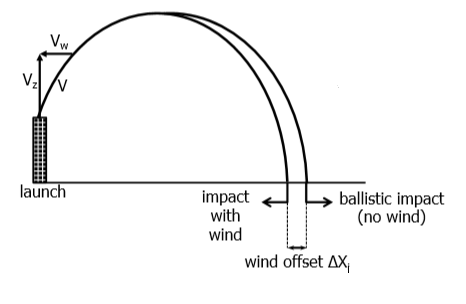
\includegraphics[scale=1]{4c}

Wind offset can be computed in the following way
$$wind\:\: offset = V_wt_{flight} = 10\times360 = 3600\: m$$
\end{enumerate}